\documentclass[fleqn,10pt]{wlscirep}
\usepackage[utf8]{inputenc}
\usepackage[T1]{fontenc}
\usepackage{listings}
\usepackage{algorithm2e}

\title{AGEAS: Automated Machine Learning based Genetics Featrue Extraction System}

\author[1,2,*1,+]{Jack Yu}
% \author[1,2,*1]{Jack Yu}
\author[2,+]{Masayoshi Nakamoto}
\author[1,*2,+]{Jiawang Tao}

% \author[2,+]{Derek Author}
\affil[1]{Center for Health Research, Guangzhou Institutes of Biomedicine and Health, Chinese Academy of Sciences, Guangzhou 510530, China}
\affil[2]{Shenzhen Mozhou Technology Co., Ltd, Shenzhen, China}
% \affil[2]{Affiliation, department, city, postcode, country}
\affil[*1]{Correspondence: gyu17@alumni.jh.edu}
\affil[*2]{Correspondence: tao\_jiawang@gibh.ac.cn}

\affil[+]{these authors contributed equally to this work}
\keywords{Machine Learning, Gene Regulatory Network, RNA-Seq, Chip-Seq}

\begin{abstract}
  Abstract goes here
\end{abstract}

\begin{document}
\flushbottom
\maketitle

\thispagestyle{empty}
% \noindent Please note: Abbreviations should be introduced at the first mention in the main text – no abbreviations lists. Suggested structure of main text (not enforced) is provided below.

\section*{Introduction}


\section*{Method}
  \label{method}
  The basic principle of \emph{AGEAS} is to find key genetic features regulating phenotype of interest through analyzing how well-performing classification models distinguish gene regulatory networks (GRNs) of sample with the phenotype from GRNs of samples.
  To reconstruct sufficient GRNs for each class, RNA-seq based expression data is segmented into subsets while each one is analogized as a pseudo-sample having discrete expression data.
  The pseudo-sample GRNs (psGRNs) are reconstructed accordingly; thus, classification models can be trained, evaluated, and interpreted having gene regulatory pathways (GRPs) as input factors.
  With heavily weighted GRPs and associated genes repeatedly obtained from interpretations of success sample class predictions, regulons could be formed and inferred as genetic feature complexes playing important role in differentiating the studying sample classes.
  The overall workflow can be summarized as Figure \ref{workflow}.
  Following sections describe each step of \emph{AGEAS} in more depth.
  % \begin{itemize}
  %   \item \hyperref[step1]{\textbf{\emph{Step 1}}}: Data preprocessing
  %   \item \hyperref[step2]{\textbf{\emph{Step 2}}}: Classification model selection.
  %   \item \hyperref[step3]{\textbf{\emph{Step 3}}}: Feature selection...
  %   \item \hyperref[step4]{\textbf{\emph{Step 4}}}: Top GRP extraction.
  %   \item \hyperref[step5]{\textbf{\emph{Step 5}}}: Key network reconstruction.
  % \end{itemize}
  \begin{figure}[ht]
  \centering
  % 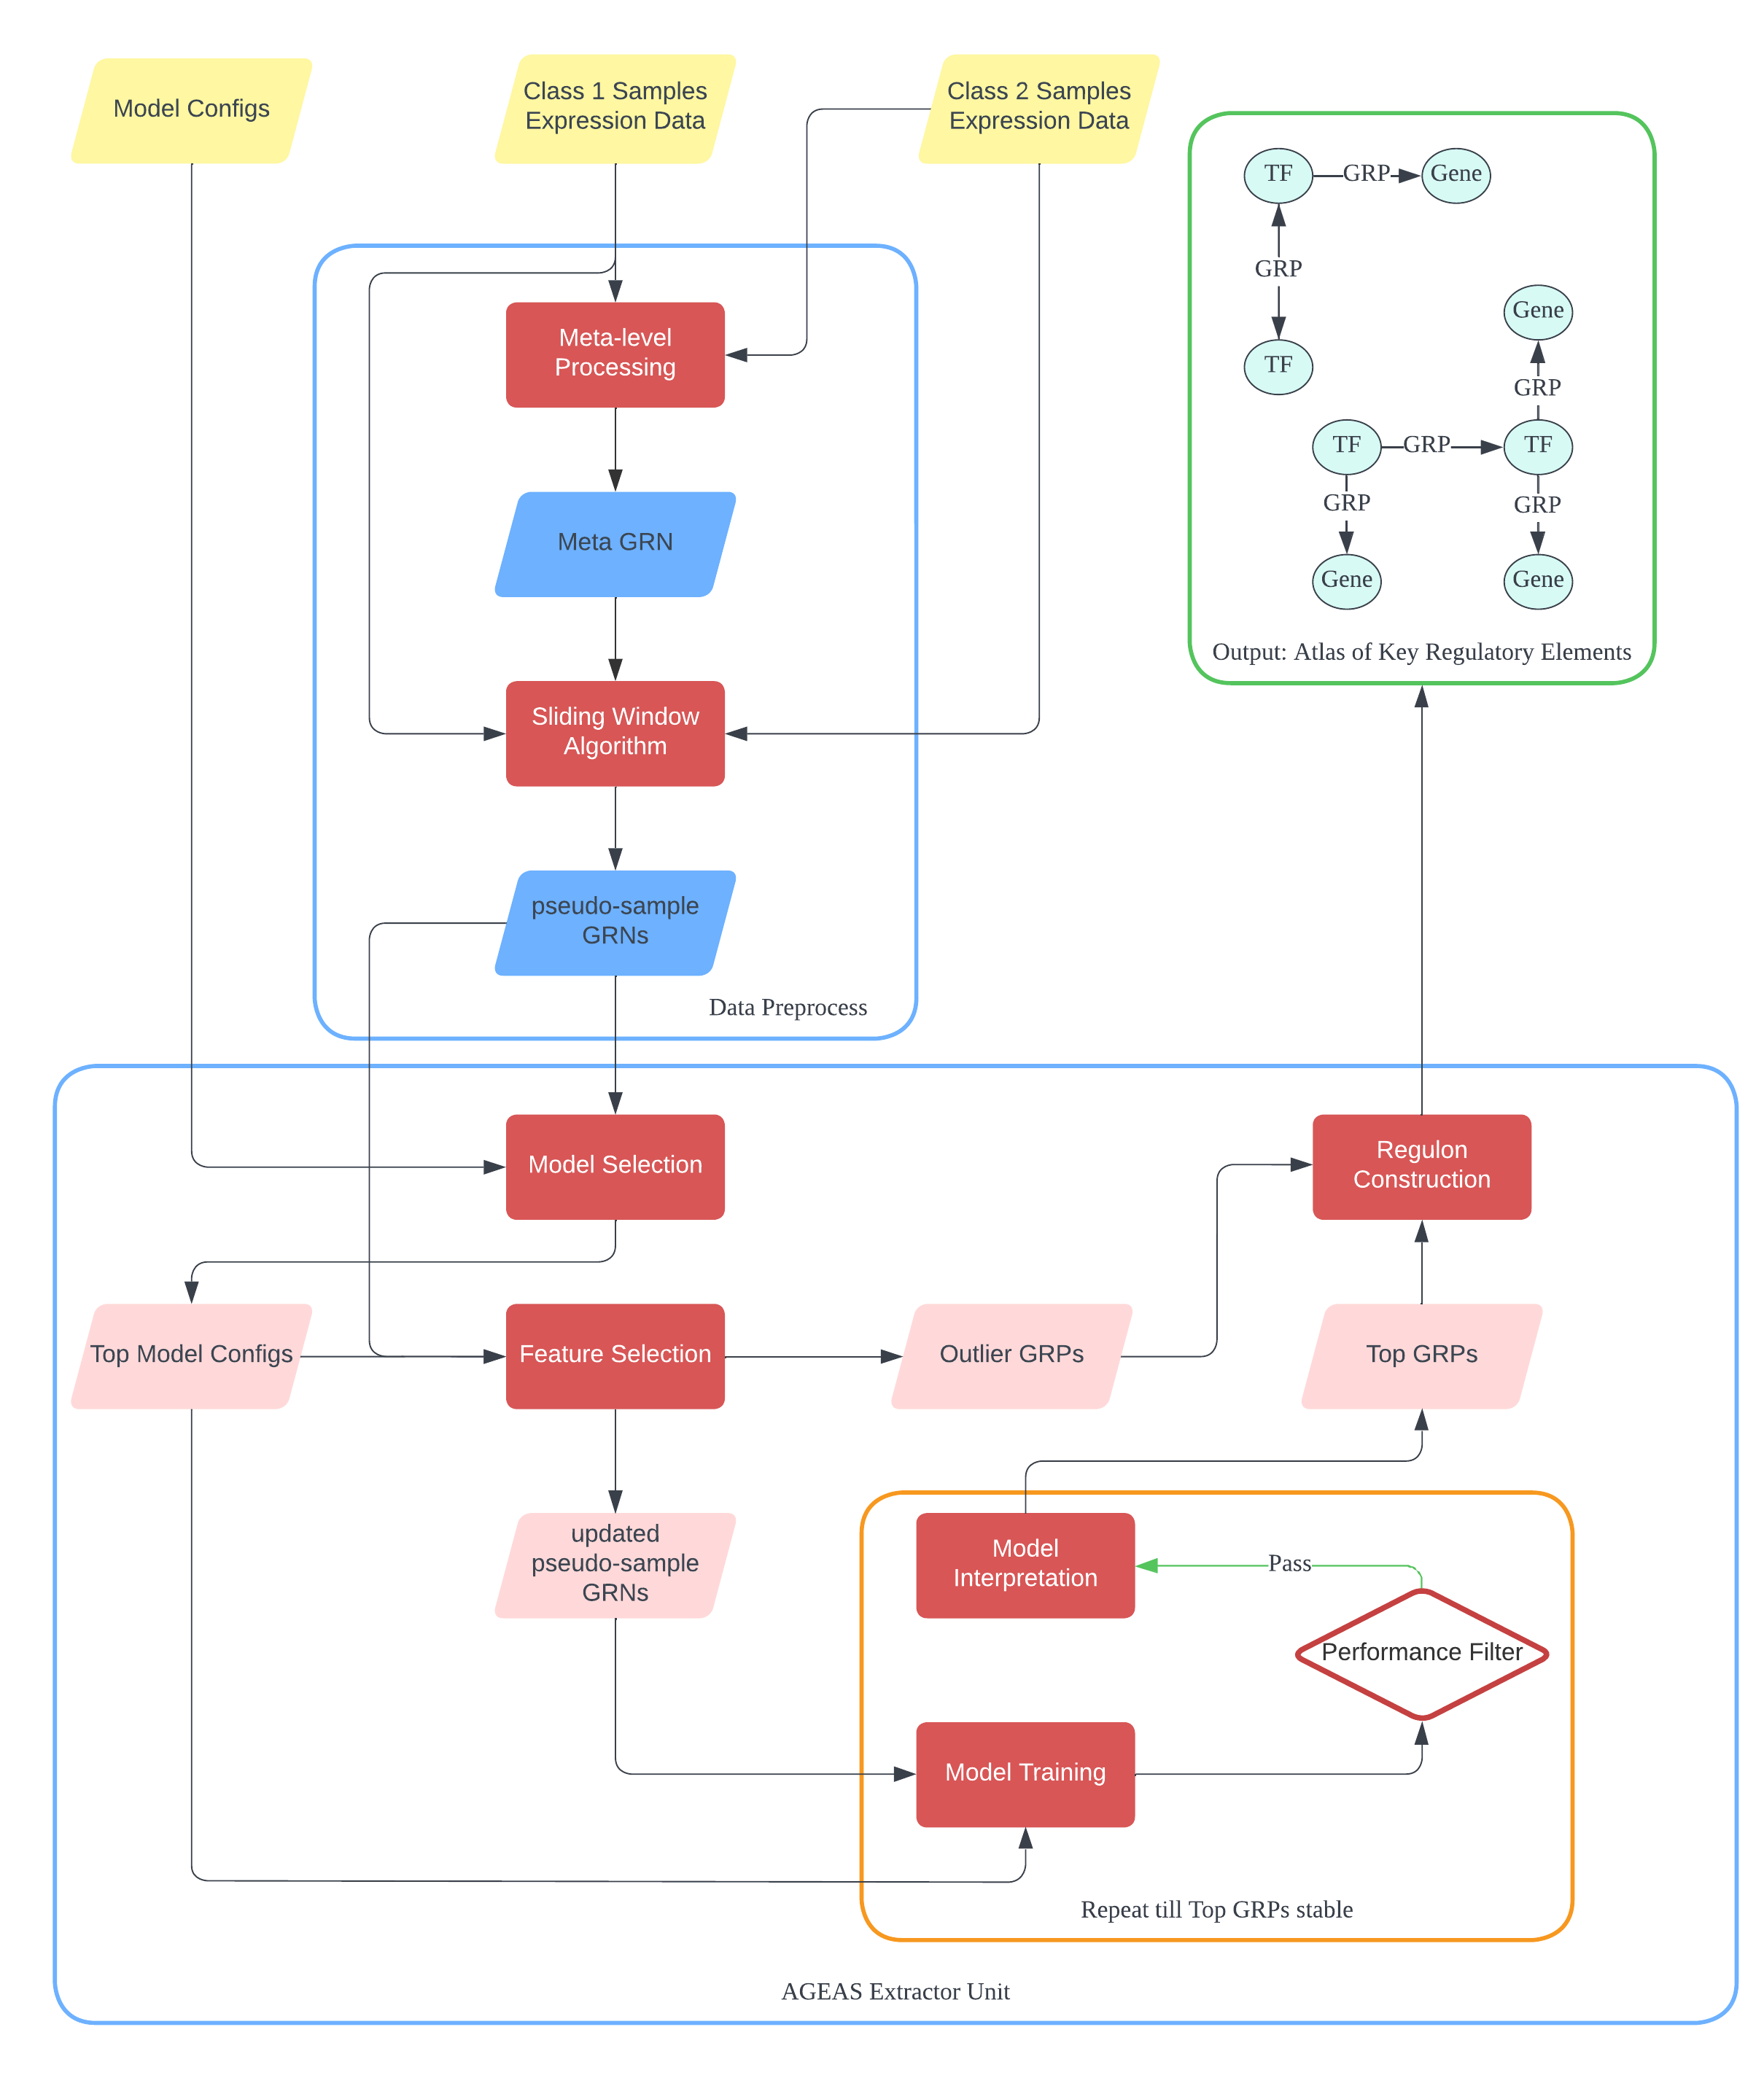
\includegraphics[width=0.8\linewidth, height=18cm, keepaspectratio,]{../images/summary_trans.png}
  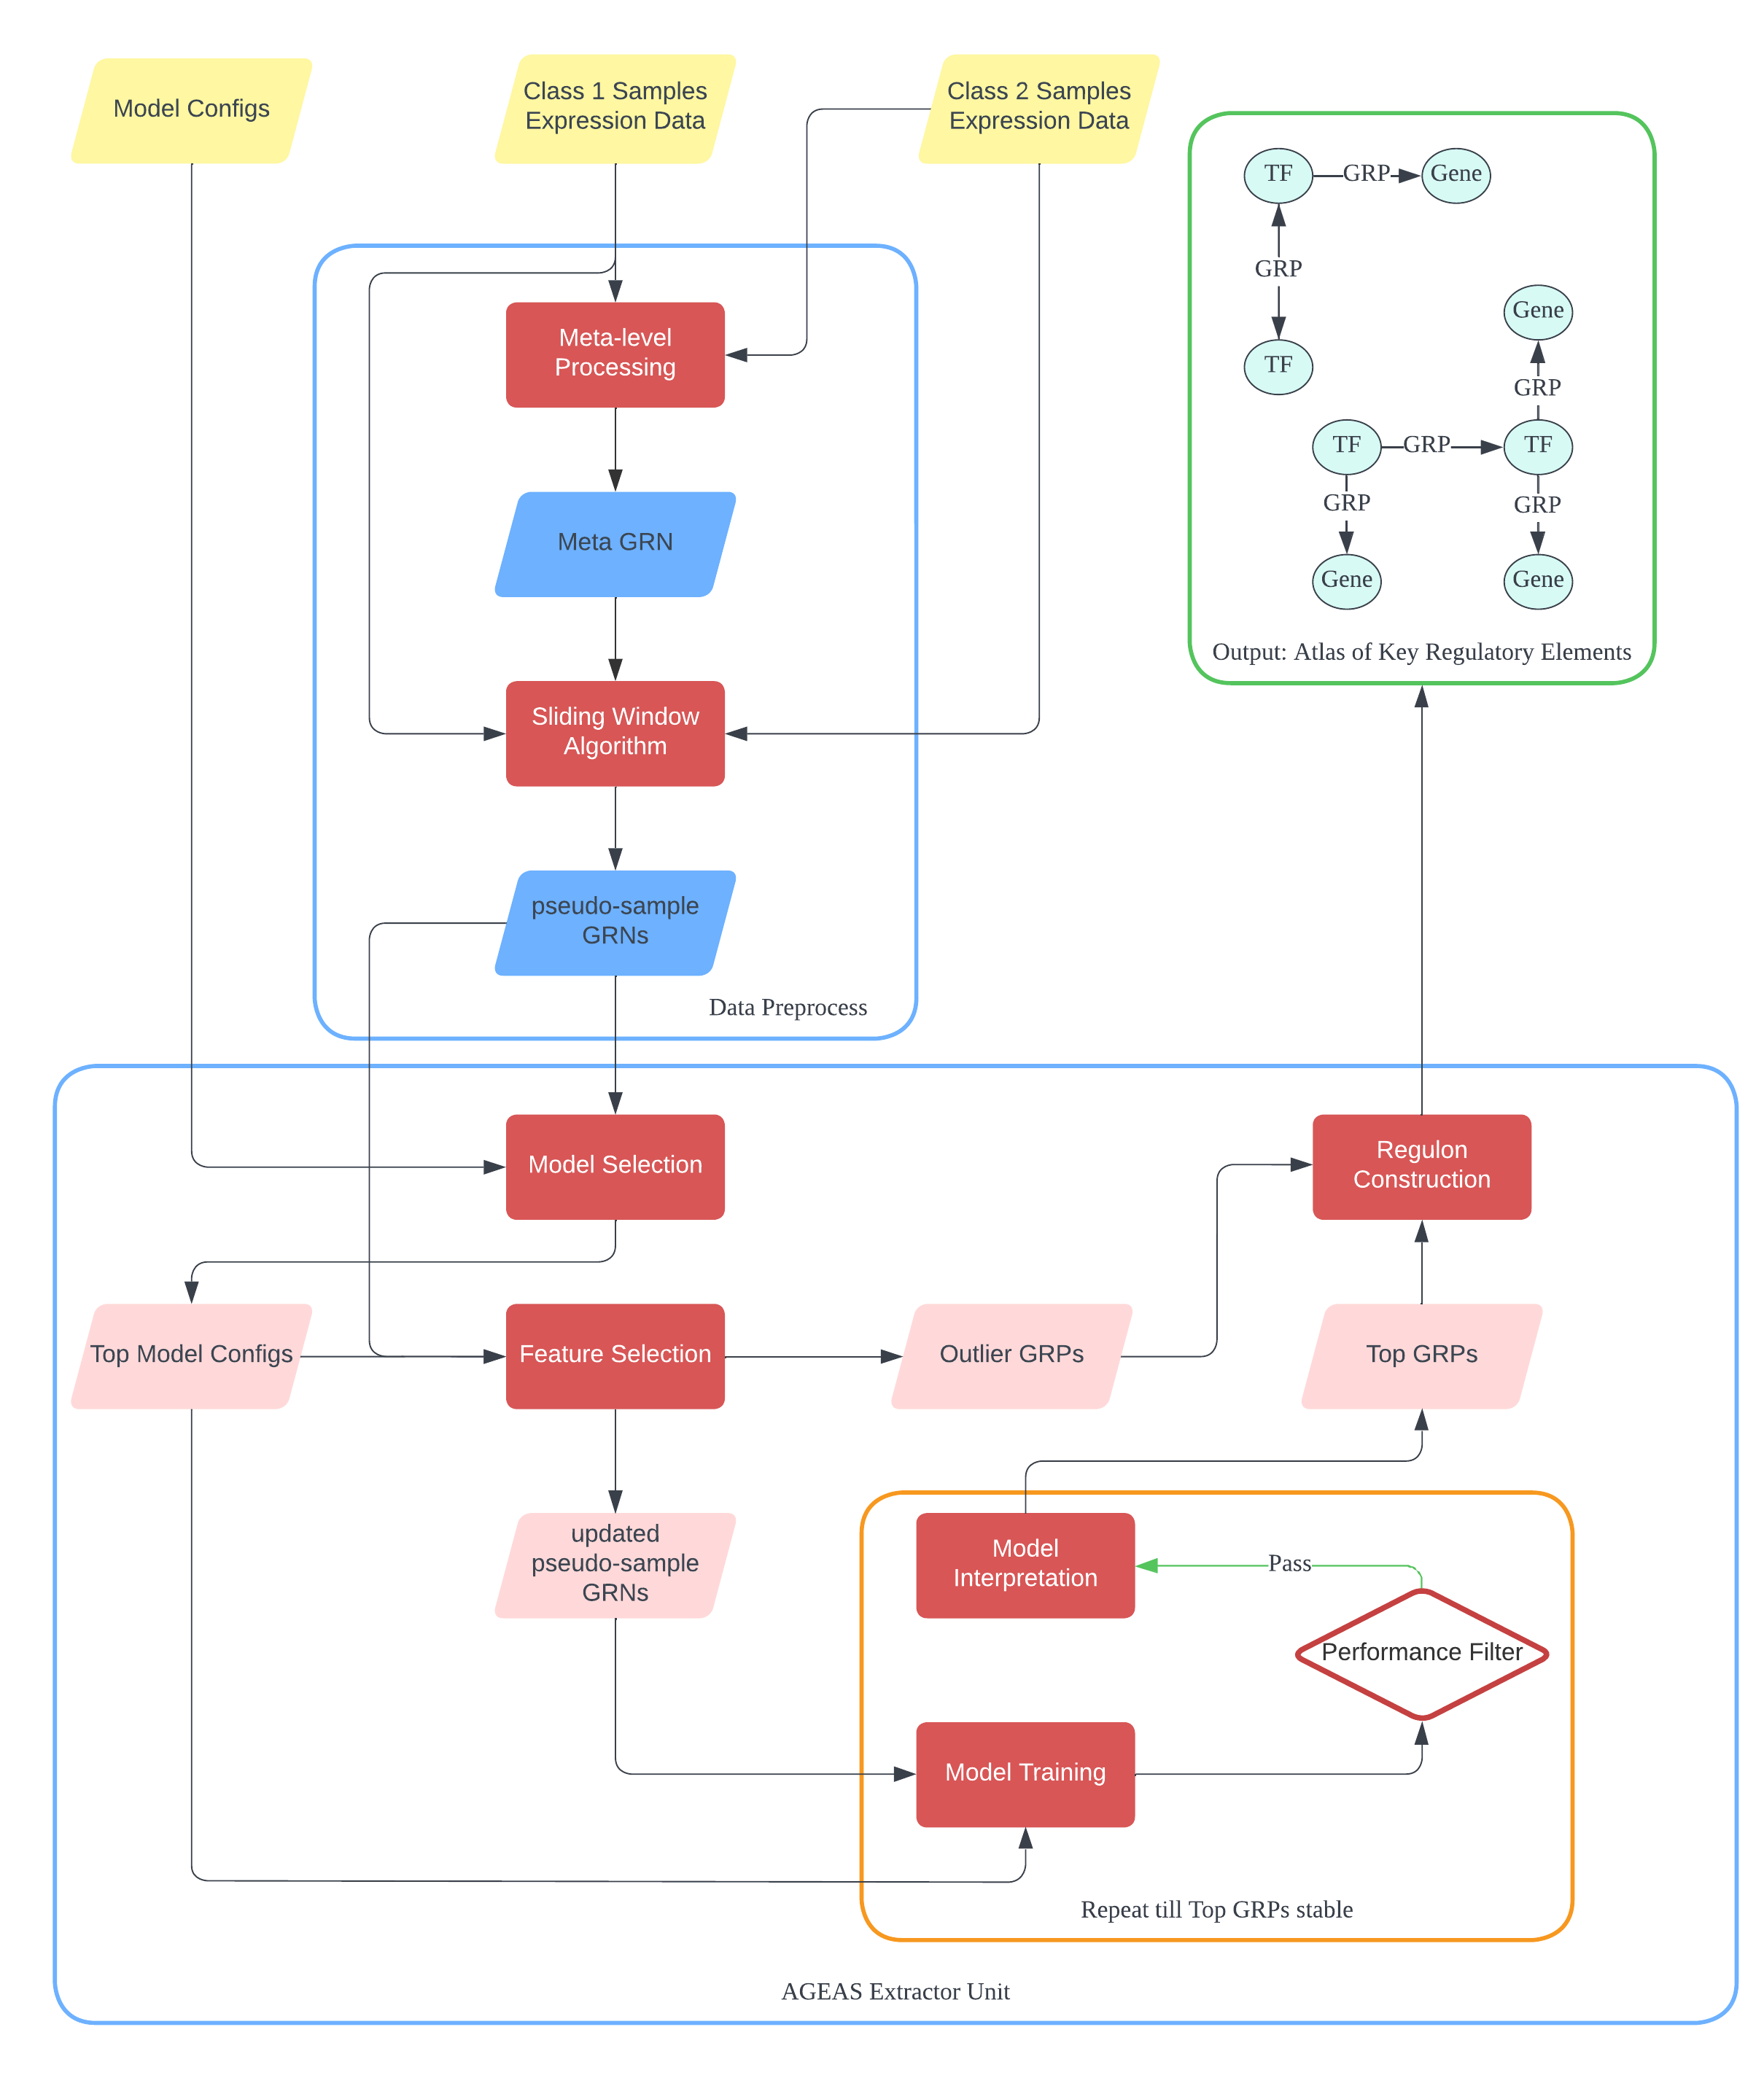
\includegraphics[width=0.8\linewidth, keepaspectratio,]{../images/summary_trans.png}
  \caption{
    The overall workflow of \emph{AGEAS}:
    \textbf{\emph{(1)}} Reconstruct meta-level GRN (meta-GRN) with expression data of all samples.
    \textbf{\emph{(2)}} Build pseudo-samples with sliding window algorithm and reconstruct GRNs with GRPs identified in meta-GRN accordingly.
    \textbf{\emph{(3)}} Select best performing classifiers in predicting class labels of pseudo-sample GRNs (psGRNs).
    \textbf{\emph{(4)}} Interpret how top models make classifications and gradually exclude GRPs with low weights or outlier-level high weights.
    \textbf{\emph{(5)}} Repeatedly train classifiers with differnt set of psGRNs as training data to extract GRPs frequently ranked as top important features for decision.
    \textbf{\emph{(6)}} Reconstruct regulons with extracted GRPs and GRPs excluded as significant outliers.
  }
  \label{workflow}
  \end{figure}

  \subsection*{Step 1:Data preprocessing}
    \label{step1}
    The main purpose of this step is to build pseudo-samples and reconstruct corresponding pseudo-sample GRNs (psGRNs).
    % Instead of finding genes being important to differentiate sample classes and infer gene regulatory networks (GRNs) with the genes,
    For each sample class, gene expression matrices (GEMs) labeled with same class label are concatenated as one comprehensive expression matrix.
    With comprehensive GEMs, a meta-level GRN (meta-GRN) is reconstructed in advance of psGRNs to provide generic guidance on reconstruction.
    In general, the workflow of this step can be represented as Figure \ref{data_preprocess}.

    \subsubsection*{Reconstruct meta-GRN}
      Firstly, genes included in the comprehensive GEMs are assessed and determined whether having potential to form informative GRPs with other genes.
      Commonly, differentially expressed genes (DEGs) would be considered as important factors of studying feature.
      Here we apply the Mann-Whitney U rank test (MWW) implemented by \emph{SciPy}\cite{2020SciPy-NMeth} to exclude genes having indistinguishable expression level distribution across GEMs of different classes.
      The p-value for rejecting null hypothesis, that expression distribution underlying class 1 samples is the same as the expression distribution underlying class 2 samples, is set to 0.05 by default.
      Furthermore, a $\log_2$ fold change (log2FC) filter is also implemented in \emph{AGEAS}.
      However, enabling the log2FC filter is not encouraged considering upstream transcription factors (TFs) indirectly regulating key genes associated with feature of interest may not always have significant expression level difference between sample classes.
      The lof2FC filter shall mostly be used in order to decrease meta-GRN's GRP total amount in a compromising position caused by limited computational resources.
      After differential expression based filters, a standard deviation ($\sigma$) filter is applied to exclude genes either having low expression value or merely affected by dynamic expression status of other genes.
      By default, the $\sigma$ threshold is set to 1.0 consisting with the lowest expression level in raw gene count matrix gained from RNA-Seq data.
      The threshold value should be adjusted corresponding to prior knowledge of input GEMs, for example of what normalization method was applied to the GEMs.

      With candidate genes passed filters above, some gene pairs are formed and assessed potential of representing GRPs.
      To reduce overall computational complexity, a gene pair shall be formed with at least one TF which could be the regulatory source of GRP.
      If not further specified, TF list will be retrieved from integrated \emph{TRANSFAC}\cite{transfac} datasets according to the provided species information.
      Utilizing genetic interaction database like \emph{GTRD}\cite{gkaa1057} and \emph{BioGRID}\cite{biogrid}, \emph{AGEAS} checks whether the binding ability of gene pair is confirmed or not.
      By default, if TF being recorded to have binding site within target gene's promoter range (-1000 to +100) by Chip-Seq dataset retrieved from \emph{GTRD}\cite{gkaa1057}, the potential GRP gene pair will be passed to expression correlation assessment.
      For TFs not covered by interaction database, \emph{GRNBoost2}\cite{grnboost2}-like algorithm is initiated to predict potential regulatory target genes.
      The prediction importance threshold can either be set manually or automatically based on recorded interactions as:

      \centerline{$Threshold = min(GA(M_1, t)\, \uplus \, GA(M_2, t), \frac{1}{g})$}

      \noindent Here $GA()$ denotes \emph{GRNBoost2}\cite{grnboost2}-like algorithm;
      $M_1$ is concatenated class 1 samples GEM with genes passed filters;
      $M_2$ is concatenated class 2 samples GEM with genes passed filters;
      $t$ is the TF having largest amount of recorded interaction in dataset;
      $g$ is total amount of unique genes in all samples passed filters.

      After potential GRP gene pairs obtained, a expression correlation filter is used to exclude gene pairs having low covariance which implies weak relationship.
      To assess expression correlation, \emph{AGEAS} applies Pearson's Correlation coefficient\cite{pcc_2012} (PCC) whihc is one of the widely adopted methods\cite{cid_2019}.
      With default setting, gene pairs can reach absolute correlation coefficient of 0.2 while keeping correspond p-value lower than 0.05 are included in meta-GRN as validated GRP.

    \subsubsection*{Reconstruct psGRNs}
      The comprehensive GEMs is divided into few sample subsets with sliding window algorithm (SWA) to build pseudo-samples.
      With SWA, we can gain GEM of \emph{i-th} pseudo-sample through:

      \centerline{$SWA(i) = \left\{{x_j}_{j = i * p}^{j + k}\right\}, j + k < l$}

      \noindent Here $l$ is number of samples in a comprehensive GEM which can be expressed as $\left\{{x_j}_{j = 0}^{l}\right\}$; $k$ denotes window size; $p$ denotes padding stride.

      If sample amount is considerably low or imbalanced, customized window size and padding stride can be applied to generate sufficient amount of pseudo-samples for later classifier training and assessment processes.
      Utilizing meta-GRN, psGRNs are reconstructed with GEMs of pseudo-sample.
      Each GRP gene pair in meta-GRN is formed with expression data in pseudo-sample and filtered by same PCC filter in meta-GRN reconstruction process.
      After all pseudo-samples have been used to reconstruct psGRN, every psGRN will have GRP rearranged by unified order.

    \begin{figure}[ht]
      \centering
      % 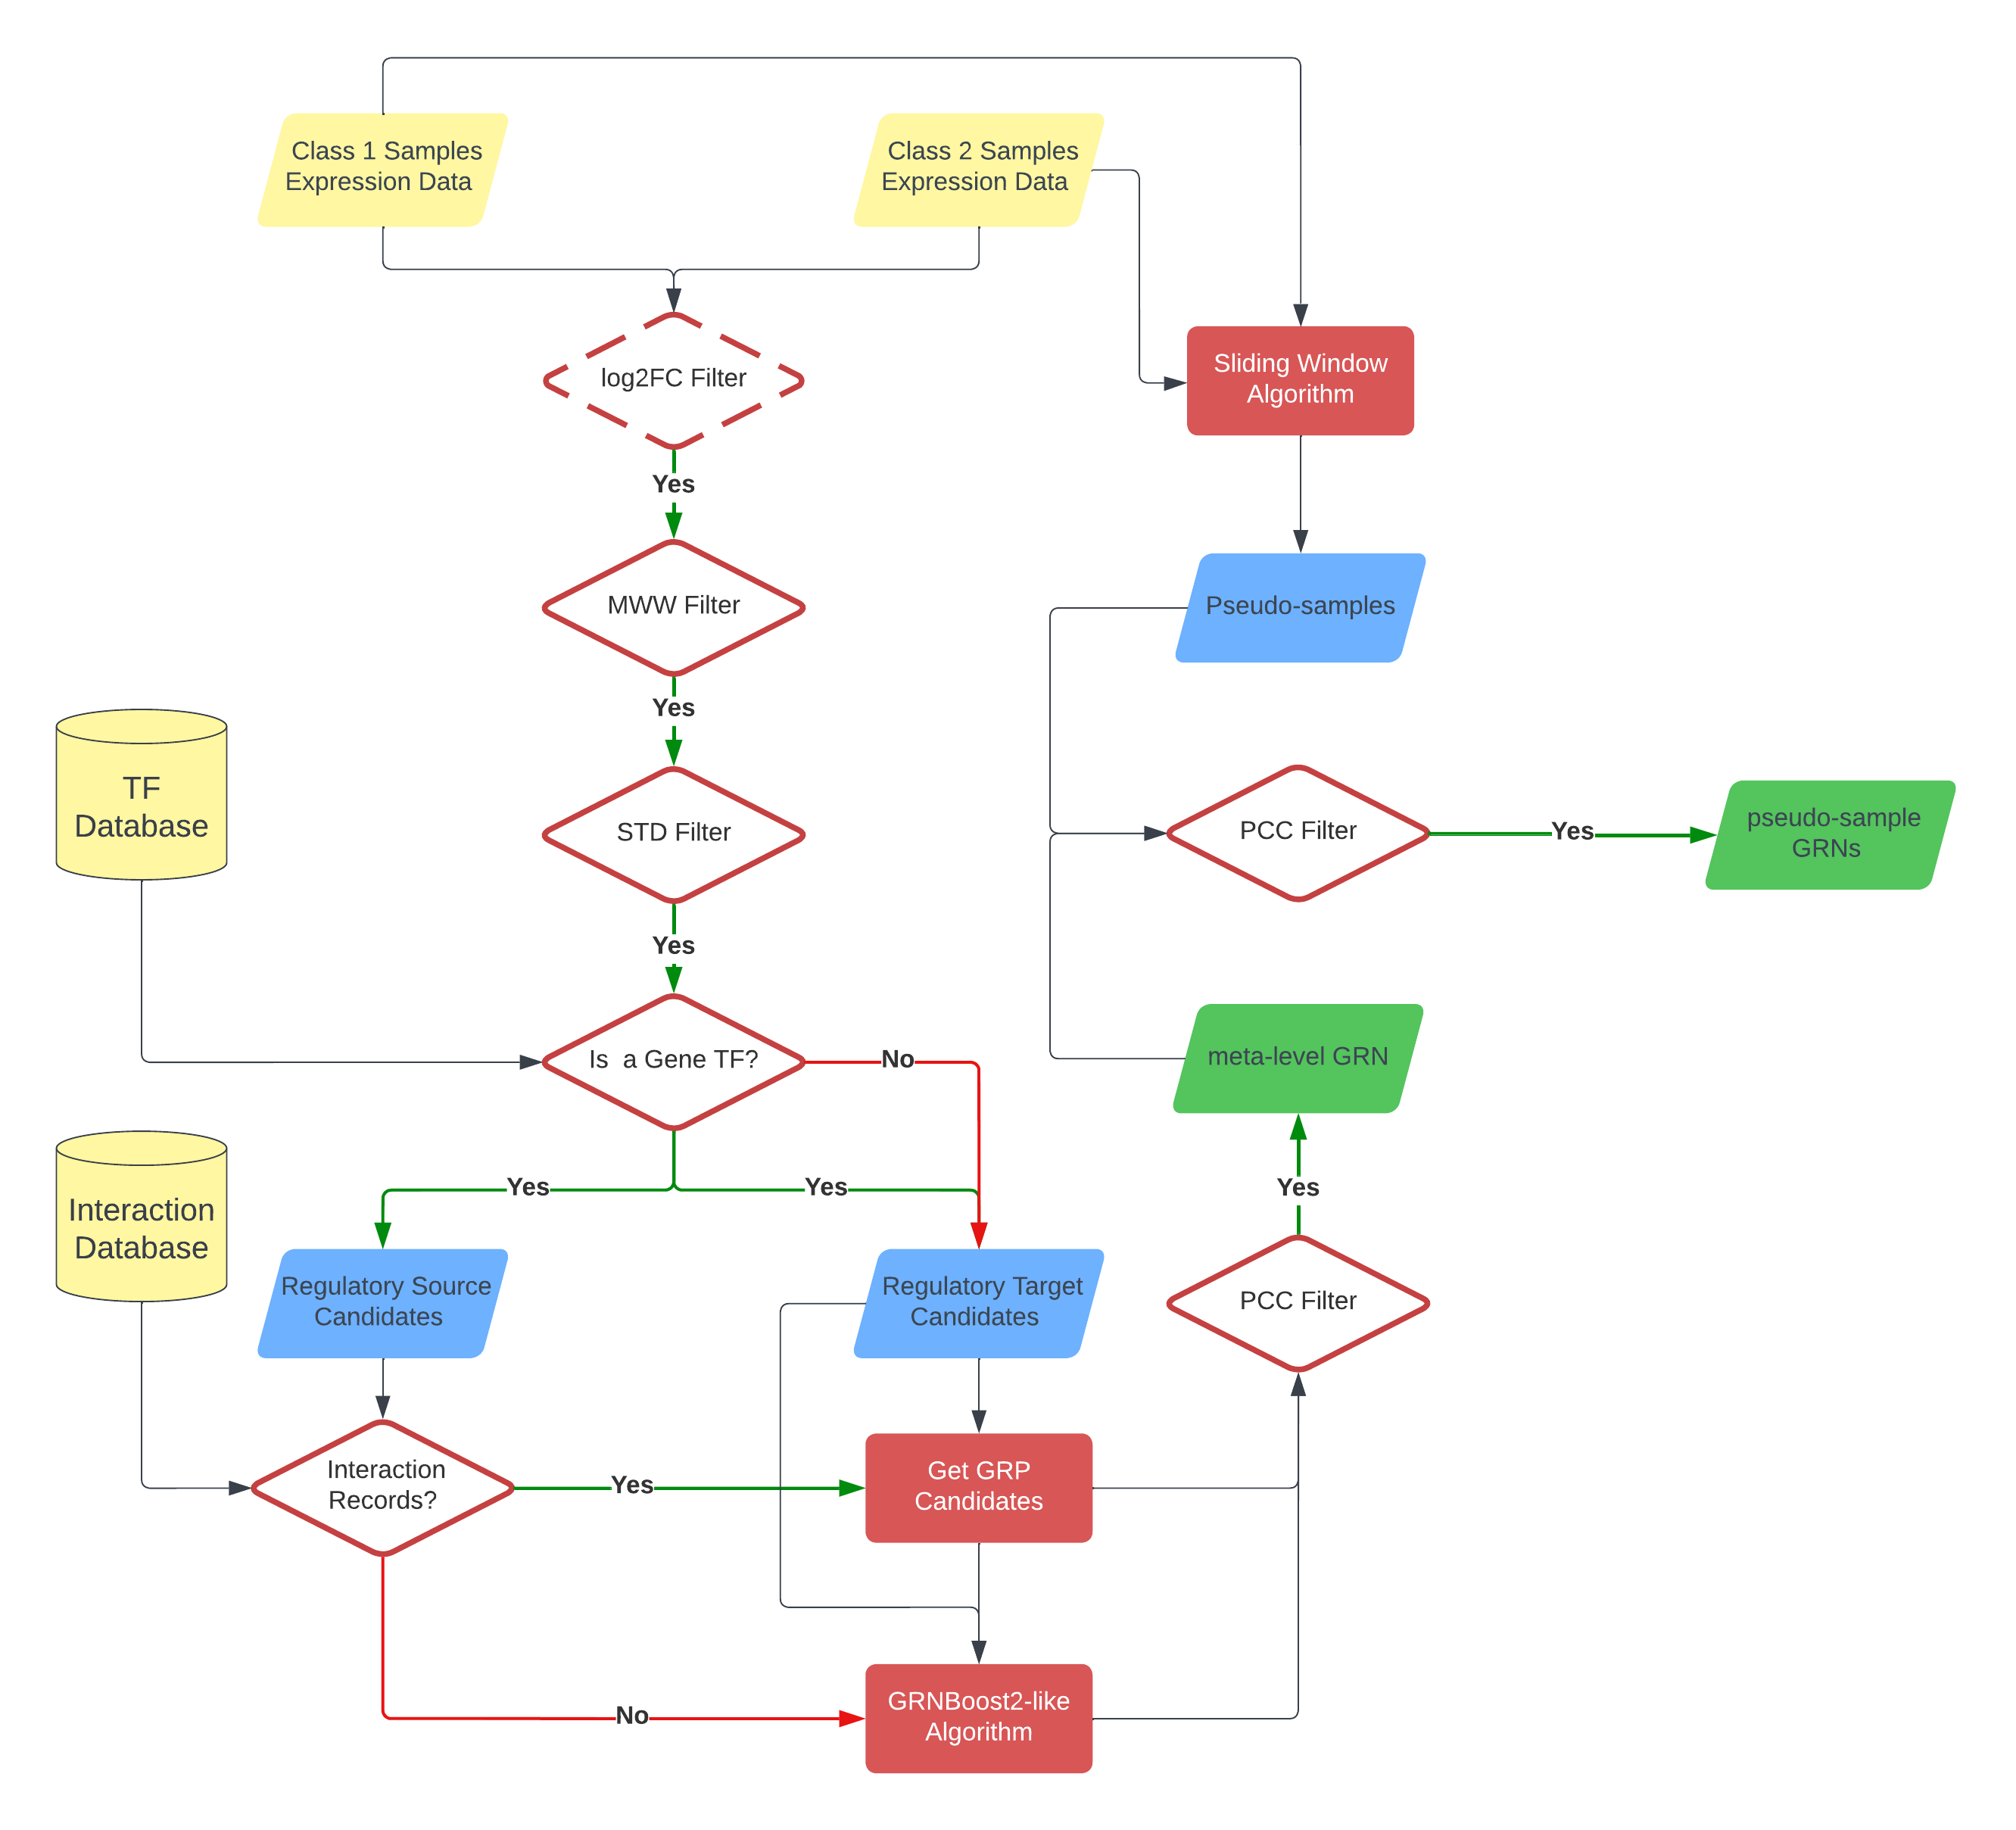
\includegraphics[width=0.8\linewidth, height=12cm, keepaspectratio,]{../images/data_preprocess_trans.png}
      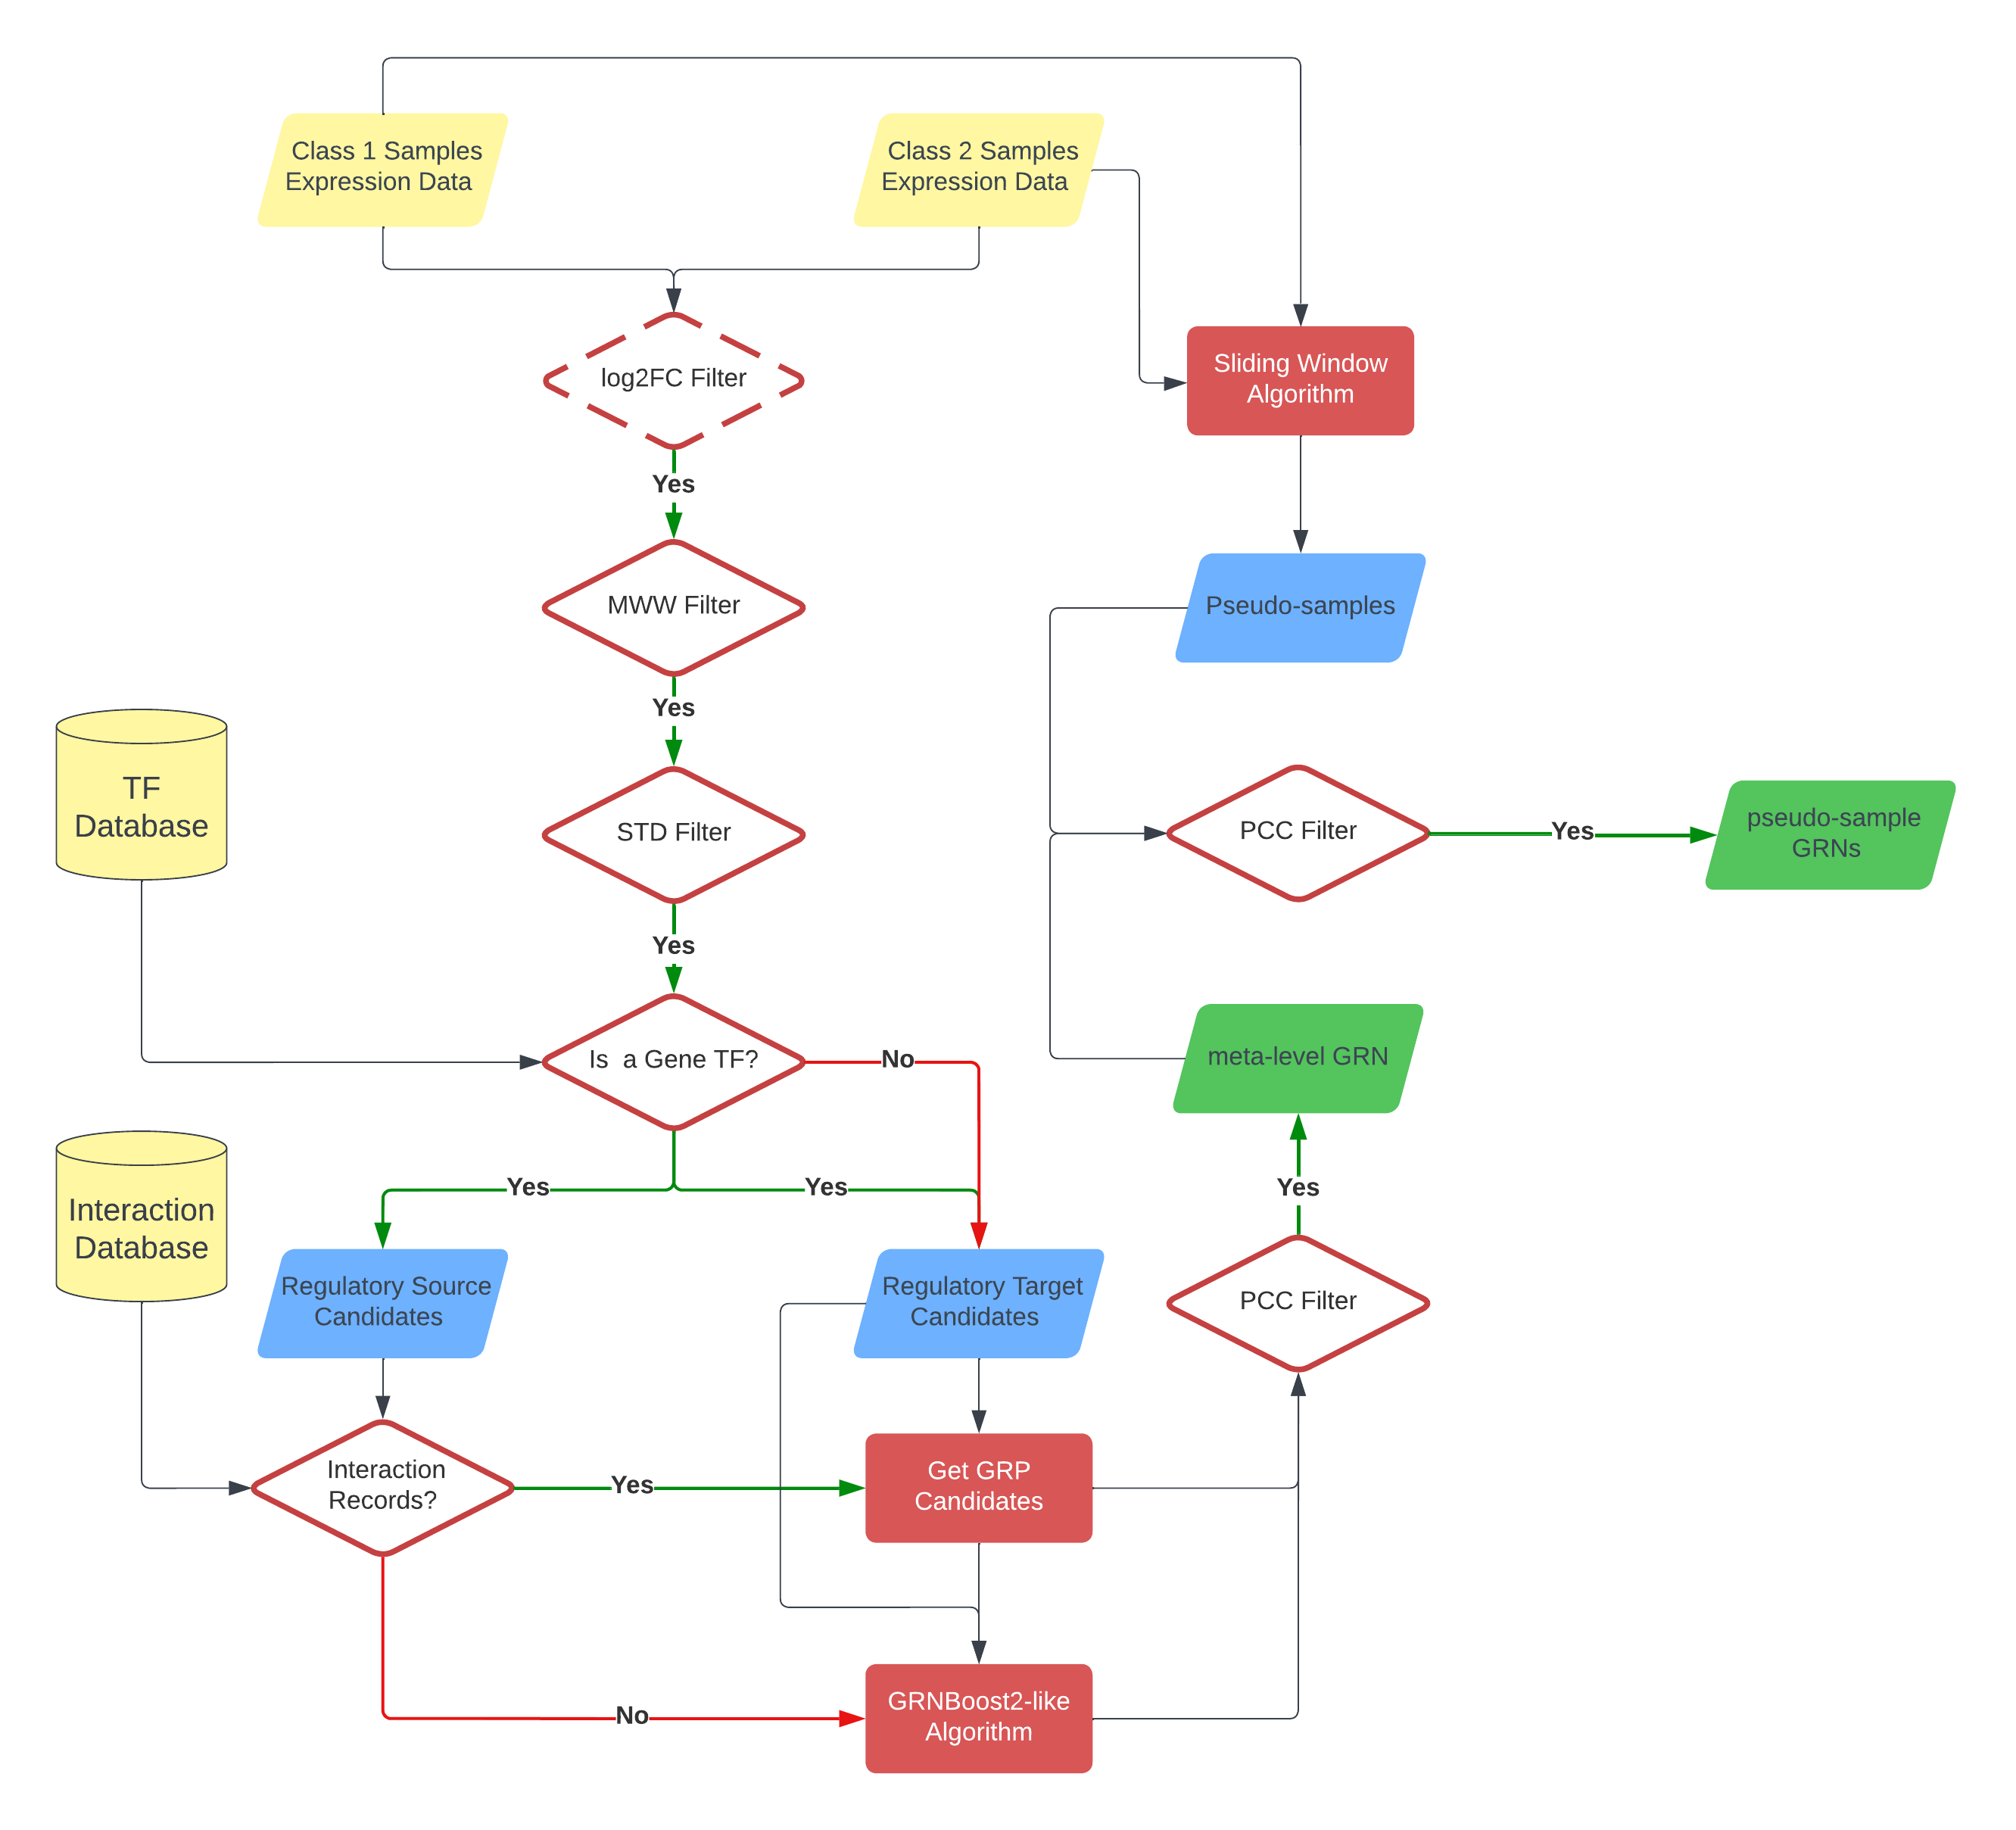
\includegraphics[width=0.8\linewidth, keepaspectratio,]{../images/data_preprocess_trans.png}
      \caption{
        Workflow to reconstruct meta-GRN and psGRNs.
        \textbf{\emph{(1)}} Filter genes from GEMs with log2FC filter(optional), MWW filter, and $\sigma$ filter.
        \textbf{\emph{(2)}} Find candidate GRP gene pairs from either interaction database or predictions made by \emph{GRNBoost2}\cite{grnboost2}-like algorithm.
        \textbf{\emph{(3)}} Filter candidate GRP gene pairs with PCC filter and reconstruct meta-GRN with validated GRPs.
        \textbf{\emph{(4)}} Generate pseudo-samples with SWA.
        \textbf{\emph{(5)}} Utilize GRPs in meta-GRN as generic guidance to form candidate GRPs for pseudo-samples.
        \textbf{\emph{(6)}} Filter every candidate GRP for all pseudo-samples with PCC filter and reconstruct psGRNs with validated GRPs.
      }
      \label{data_preprocess}
    \end{figure}

  \subsection*{Step 2: Classification model selection}
    \label{step2}
    Since \emph{AGEAS} is not aiming to develop optimized model architectures for psGRN classification but gain insights from multiple models as divergent as possible, the main goal of this step is to select configurations of models capable to make correct psGRN classifications from provided configuration set.
    Regarding the fact that computational power is limited resource, portion of less efficient model configurations shall be pruned although interpreting success predictions of more classification models would lead to more comprehensive insight into sample class differences.
    Therefore, we apply a simple Hyperband\cite{hyperband}-based algorithm \ref{alg:one} which performs grid search for well-performing classification models with varying model training resource and pruning aggressiveness.


    %% This declares a command \Comment
    %% The argument will be surrounded by /* ... */
    \SetKwComment{Comment}{/* }{ */}
    \SetKwInput{kwInput}{Input}
    \SetKwInput{kwReturn}{Return}
    \RestyleAlgo{ruled}
    \begin{algorithm}
    \caption{Model selection algorithm}
    \label{alg:one}
    \kwInput{$R, C, I$ (default $I = 3$), $\alpha_{max}$(default $\alpha_{max} = 0.9$),  $k_{min}$(default $k_{min} = 0.5$)}
    $\alpha_{low} = \frac{1}{(2 ^ {I} - 1)}$\;
    % $X \gets x$\;
    \For{$i \in \{0, 1, ..., I-1\}$}{
      \eIf{$i == I-1$}{
        $\alpha = \alpha_{max}$\;
        % $X \gets X \times X$\;
        % $N \gets \frac{N}{2}$
        % \Comment*[r]{This is a comment}
      }{
        $alpha = 2^i \alpha_{low}$\;
      }
      $r = \alpha R$\;
      $P = \emptyset $\;
      \For{$c \in C$}{
        $p = run\_then\_evaluate(c, r, R)$\;
        Append $p$ to $P$\;
      }
      % \If{$N$ is odd}{
      %   }

      $k = max(1 - \alpha, k_{min}$)\;
  	  $C = top\_configs(C, P, k$)\;
    }
    \kwReturn{$C$}
    \end{algorithm}

    The model selection algorithm requires five inputs
    (1)$R$, the maximum amount of training resource, equivalent to all avaliable psGRNs
    (2)$C$, the total set of provided classification model configurations
    (3)$I$, the number of iterations for model pruning (default set as 3)
    (4)$\alpha_{max}$, the maximum portion of $R$ can be fed to single model (default set as 0.95)
    (5)$k_{min}$, the minimum portion of remaining model configurations will be kept by single pruning iteration (default set as 0.5).
    Furthermore, two functions are also required while need to be defined based on input model configurations:
    \begin{itemize}
    \setlength\itemsep{0em}
    \item \textbf{$run\_then\_evaluate(c, r, R)$}: trains classification model initialized using configuration $c$ for the allocated resource $r$, then returns prediction accuracy (ACC), the area under a receiver operating characteristic curve (AUROC)\cite{hanley_mcneil_1982} score, and total cross-entropy loss ($L_{CE}$) calculated through predicting sample class for all psGRNs $R$.

    \item \textbf{$top\_configs(C, P, k)$}: takes a set of model configurations $C$ with associated evaluation results $P$ and returns configurations having ACC, AUROC score, or $L_{CE}$ reaching top $k$ portion.
    \end{itemize}

    \noindent By default, \emph{AGEAS} initializes with 128 model configurations utilizing 9 integrated classification algorithms listed in Table \ref{models}.

    \begin{table}[ht]
      \centering
      \begin{tabular}{|l|l|l|l|l|}
      \specialrule{.2em}{.1em}{.1em}
      \textbf{Algorithm} & \textbf{$\# \lambda$} & \textbf{Categorical} & \textbf{Continuous} & \textbf{$\#$ Configs}\\
      \specialrule{.2em}{.1em}{.1em}
      \multicolumn{5}{|l|}{\emph{Implemented with Pytorch}\cite{NEURIPS2019_9015}} \\
      \hline
      Transformer & \textbf{14} & 4 & 10 & 32 \\
      \hline
      1D Convolutional Neural Network (1D-CNN) & \textbf{10} & 2 & 8 & 32 \\
      \hline
      Hybrid Convolutional Neural Network (Hybrid-CNN) & \textbf{10} & 2 & 8 & 32 \\
      \hline
      Gated Recurrent Unit (GRU) & \textbf{10} & 4 & 6 & 4 \\
      \hline
      Long Short-Term Memory (LSTM) & \textbf{11} & 4 & 7 & 4 \\
      \hline
      Standard Recurrent Neural Network (RNN) & \textbf{11} & 5 & 6 & 4 \\
      \specialrule{.2em}{.1em}{.1em}
      \multicolumn{5}{|l|}{\emph{Implemented with XGBoost}\cite{chen2016xgboost}} \\
      \hline
      Gradient Boosted Decision Trees (GBDT) & \textbf{18} & 5(1) & 13(4) & 16 \\
      \specialrule{.2em}{.1em}{.1em}
      \multicolumn{5}{|l|}{\emph{Implemented with scikit-learn}\cite{scikit-learn}} \\
      \hline
      Random Forests (RF) & \textbf{14} & 5(1) & 9(1) & 2 \\
      \hline
      Support Vector Machine (SVM) & \textbf{7} & 4 & 3(3) & 2 \\
      \specialrule{.2em}{.1em}{.1em}
      \end{tabular}
      \caption{
        \label{models}
        Classification model algorithms integrated in \emph{AGEAS} with correspond numbers of hyperparameter and preset model configurations.
        Categorical hyperparameters and continuous numerical hyperparameters are clarifed beside total number of hyperparameters ($\# \lambda$).
        Conditional hyperparameters which are required for selected other hyperparameters are shown in brackets if there is any.
        $\#$ Configs indicates total amount of configurations \emph{AGEAS} applies by default.
      }
    \end{table}

    The general architecture designs of 1D-CNN and Hybrid-CNN are implemented referring to 1D-CNN and 2D-Hybrid-CNN applied in recent cancer type prediction study\cite{mostavi_chiu_huang_chen_2020}.
    However, taking one convolution layer and adjacent max-pooling layer as a layer set, we implemented both CNN models with flexibilities on number of layer set, which is fixed as 1 in original research.
    An example of 1D-CNN with 2 convolution layer sets is illustrated in Figure \ref{1dCNN}.

    \begin{figure}[ht]
      \centering
      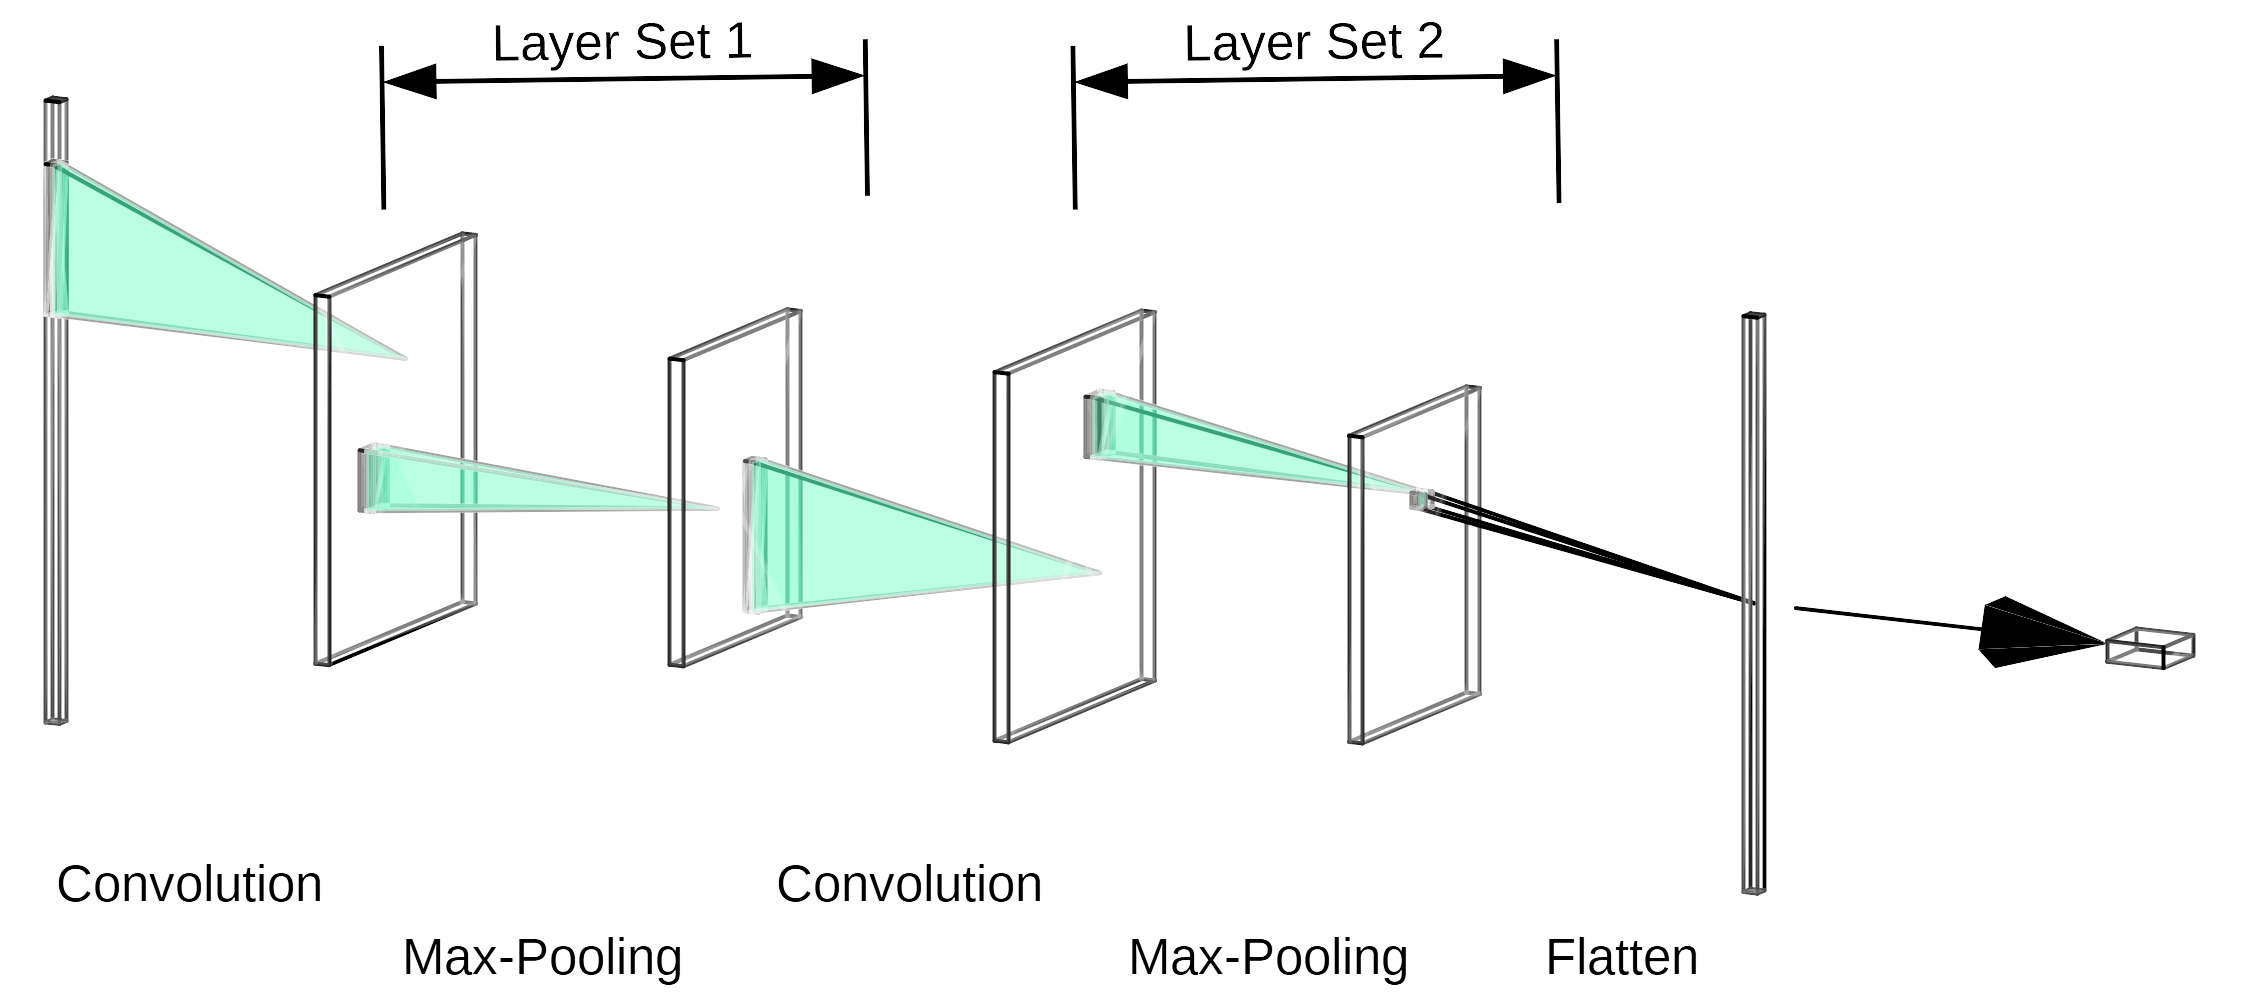
\includegraphics[width=0.8\linewidth]{../images/nn.png}
      \caption{1D-CNN with 2 convolution layer set.}
      \label{1dCNN}
    \end{figure}

    For transformer models, considering psGRNs are already be represented by numerical data matrix while GRPs should barely have positional relationships in the matrix, the embedding layer and positional encoding layer designed for input data tokenization in standard architecture \cite{transformer} are replaced with a single linear layer in \emph{AGEAS}.

  \subsection*{Step 3: Feature selection}
    \label{step3}
    With selected well-performing models, \emph{AGEAS} already can start repetition of model training and interpretation in \hyperref[step4]{Step 4} to extract key GRPs.
    However, few uninformative GRPs in training psGRNs merely relied by any model to make classification could be pruned in advance for saving computational power.
    Furthermore, to prevent classification models focusing on a small group of GRPs regardless of training psGRNs, GRPs draw excessive attention shall also be seperated from psGRNs to improve extraction comprehensiveness.
    Thus, in this step, \emph{AGEAS} iteratively train classificaion models with dynamic $\alpha_{max}$ portion of psGRNs and obtain feature importance scores as described in \hyperref[features_importances]{subsection} below to find GRPs either scored extremely high or considerably low.

    More specifically, at each iteration, GRPs having z-scores ranked as bottom $b$ portion (default set as 0.1) are discarded.
    Also, an $i$-th ranked GRP will be seperated from psGRNs and passed to \hyperref[step5]{Step 5} directly if having z-score fulfilling the condition:

    \centerline{
      $Z_{score}^{i} \ge max(Z_{score}^{thread}, \frac{Z_{score}^{i-1}}{3}, 3 \cdot IQR)$
    }

    \noindent The $Z_{score}^{thread}$ is input z-score threshold (default set as 3.0), and $IQR$ stands for interquartile range calculated by the beginning of each iteration.\
    With this criterion, \emph{AGEAS} ensures only GRPs draw significantly more attention shall be selected by each iteration despite the data distribution of varying z-score scalled importance values.

    By default, \emph{AGEAS} iterates this feature selection step for 3 times.

    \subsubsection*{Feature importance estimation}
      \label{features_importances}
      \emph{AGEAS} applies concept of The Shapley value\cite{roth_1988} for estimating importance of each input feature, equivalent to GRP of input psGRN, in any kind of classification model while making predictions.
      Specific Shapley value calculation or approximating methods are implemented with \emph{SHAP}\cite{lundberg2017unified} and applied to different algorithms as shown in Table \ref{shap}.
      Regarding the standard differences between feature importance estimating methods, we utilize \emph{softmax} function to normalize feature importances and define the normalized importance calculation function as:

      \centerline{$T(X) = softmax(\left\{ F(x) \right\}, x \in X)$}

      \noindent Here $X$ is total set of all features, and $F(x)$ is the importance estimating method of individual classification model being interpreted.\
      If the feature importances can be approached with internalized method $f(x)$, $F(x)$ is set as:

      \centerline{$F(x) = \frac{f(x)}{\sum_{x' \in X} f(x')}$}

      \noindent Otherwise, $F(x)$ is defined utilizing correctly classified input samples $S$, equivalent to psGRNs, with Shapley values $\phi$ of feature $x$ when predicting sample $s$ as class $c_1$ or class $c_2$:\

      \centerline{$F(x) = \sum_{s \in S}\frac{\left|\phi_{c_1,s}^{x}\right| + \left|\phi_{c_2,s}^{x}\right|}{2}$}

      \noindent After all selected classification models $M$ have been interpreted, we can intergrate the feature importances matrices weighted with corresponding models' $L_{CE}$ to one matrix $A$ as:\

      \centerline{
        $ A = \left\{ \sum_{m \in M}(1 - L_{CE}^{m})T_{m}(x) \right\}, x \in X $
      }

      \noindent Then, generalized importance values are obtained through z-score calculation and later sorted by descending order:\

      \centerline{
        $Z_{score} = \left\{\frac{a - \bar{A}}{\sigma_A}\right\}, a \in A$
      }

      \begin{table}[ht]
        \centering
        \begin{tabular}{|l|l|}
        \specialrule{.2em}{.1em}{.1em}
        \textbf{Algorithm} & \textbf{SHAP\cite{lundberg2017unified} Method}\\
        \hline
        Transformer & Gradient Explainer \\
        \hline
        1D-CNN & Deep Explainer \\
        \hline
        Hybrid-CNN & Deep Explainer \\
        \hline
        GRU & Gradient Explainer \\
        \hline
        LSTM & Gradient Explainer \\
        \hline
        RNN & Gradient Explainer \\
        \hline
        GBDT\textbf{*} & Tree Explainer \\
        \hline
        RF & Tree Explainer \\
        \hline
        SVM\textbf{*} & Linear Explainer / Kernel Explainer\\
        \specialrule{.2em}{.1em}{.1em}
        \end{tabular}
        \caption{
          \label{shap}
          Classifier algorithms with applicable Shapley value approximating methods.
          Algorithms marked with \textbf{*} have internalized feature importance estimating methods which will be applied with higher priority than Shapley value based methods.
          GBDT implemented with \emph{XGBoost}\cite{chen2016xgboost} can have feature importance approximated with average weight gain at each split involving the feature.
          Linear SVM implemented with \emph{scikit-learn}\cite{scikit-learn} can have the importance estimated with feature coefficient or using Linear Explainer.
          However, for SVM with kernel function, the feature coefficient estimation would be inappropriate, and feature importances should be approximated with Kernel Explainer.
        }
      \end{table}

  \subsection*{Step 4: Top GRP extraction}
    \label{step4}
    To extract GRPs can effectively define sample class differences, \emph{AGEAS} iteratively initializes classification models with configurations gained from \hyperref[step2]{Step 2}, trains them with varying $\alpha_{max}$ portion of psGRNs scaled after \hyperref[step3]{Step 3}, and interpret every models' correct predictions as mentioned in \hyperref[features_importances]{subsection} above.
    At each iteration, \emph{AGEAS} receives a z-score scaled feature importance matrix $A$ and add up each GRP's score accordingly from matrix $A'$ kept from previous iteration if there is one.
    Then, top $a$ (default set as 100) ranked GRPs having z-score greater than $0.0$ extracted from $A$ are compared with GRPs extracted from $A'$ by same setting.
    If less than $d$ (default set as 0.05) portion of GRPs are distinct for GRP sets stratified from $A$ and $A'$, \emph{AGEAS} will consider the GRP extration result from this iteration consists with previous one.
    Extraction iteration will terminate if either encountering $n$ (default set as 3) continuous consisting result or running out of preset iteration number (default set as 10).
    All feature importance scores in matrix $A$ from last iteration are divided by total extraction iteration number processed, and top $a$ ranked GRPs are considered as key GRPs for sample class differentiation and passed to next step.

  \subsection*{Step 5: Key network reconstruction}
    \label{step5}
    Analoging every GRP previously extracted or seperated with high z-score in \hyperref[step3]{Step 3} as a directional edge connecting two gene vertices, equivalent to a TF and a gene, in graph theory, \emph{AGEAS} attempts to reconstruct a network graph representing regulatory differences between query sample classes.
    Since there is no guarantee on all GRP edges can be connected, some regulatory relationships between gene vertices could be missed.
    Hence, \emph{AGEAS} utilizes meta-GRN gained from \hyperref[step1]{Step 1} to find GRPs which can further elucidate the regulatory relationships and adds the GRPs back to the network graph.

    For a limited iteration time (default set as  1), \emph{AGEAS} exhaustively search meta-GRN for TFs which can directly regulate any genes or TFs already covered in the network graph and add the returned TFs as new vertices.
    Next, any GRP in meta-GRN capable to connect two distinct vertices will be added if it is not covered yet.
    The network graph after expansion above represents the key genetic regulatory differences \emph{AGEAS} extracted from input sample classes.


  % With feature list ranked according to importance values, \emph{AGEAS} reconstructs regulon for top-ranked GRPs and extracts influential genes among the regulon.
  % If analoging regulon with the graph concept in discrete mathematics, one of the most common methods to analyze influence of a vertex, which is equivalent to a gene, is assessing correspond degree of the vertex.
  % Although the regulatory source and target of GRP can be determined by utilizing interaction database, such as \emph{GTRD}\cite{gkaa1057} which shows regulatory relationship of interactors, numerous computational prediction methods like \emph{GRNBoost2}\cite{grnboost2} and comprehensive interaction database, \emph{BioGRID}\cite{biogrid} for example, could not provide faithful indication on regulatory directions.
  % Consequently, based on choice of interaction database, the regulon reconstructed with \emph{AGEAS} cannot be guaranteed to be a directed graph but an undirected graph.
  % Therefore, in this step, \emph{odysseia} primarily extracts genes with high regulatory degrees in the regulon, regardless of they act as source or target in GRPs.
  % To limit total amount of output key genes, the default setting of \emph{AGEAS} reconstructs regulon for top 100 GRPs, and genes with regulatory degree higher than two in the regulon will be considered influential.
  % If regulatory directions can be clarifed, the regulatory sources capable of regulating multiple key genes and the regulatory targets influenced by multiple key genes can also be extracted according to GRN reconstruction guidance.
  %
  % In the circumstance of finding genes potentially inducing CS conversion, referred as \emph{Mogrify}\cite{mogrify_2016}, both CS deterministic genes and common regulators of these genes shall gain attention.
  % Herein, \emph{AGEAS} analogized key genes extracted from top GRPs as CS deterministic genes and TFs capable of regulating more than 2 listed key genes as significant common regulator.
  %
  % Both non-convergence issue and feature lost issue reflect on one of the key problems for $AutoML$: "No single machine learning method performs best on all datasets".\cite{NIPS2015_11d0e628}
  % Even though this problem can be solved while viewing $AutoML$ as a $CASH$ problem \cite{thornton2013auto}, such approach may not be directly deployable in our scenario considering comprehensive CS deterministic GFs or GRPs could be hardly labeled out.
  % Hence, in contrast with directly automating key features finding process, we decide to partially automate CS classification process and export candidate components of joint algorithm to feature importance analysis.
  % Compared with applying a particular $ML$ model, $CASH$ solving process during automation have higher potential to utilize comprehensive key features instead limited set of them.
  % Furthermore, due to the network-based essence of \emph{AGEAS}, some CS deterministic features failed to be detected after classification model analysis, if having close regulatory relationships with multiple confirmed GFs, can still be traced down during regulon-based analysis at post stage analysis.


\section*{Results}
  \label{res}



\section*{Discussion}
  \label{disc}


% \section*{Conclusion}
  % \label{conc}
  % Conclusion goes here

\bibliography{reference}

% For data citations of datasets uploaded to e.g. \emph{figshare}, please use the \verb|howpublished| option in the bib entry to specify the platform and the link, as in the \verb|Hao:gidmaps:2014| example in the sample bibliography file.

\section*{Author contributions statement}
\textbf{J.Y.}: Methodology, Software, Writing- Original draft preparation, Project administration
\textbf{M.N.}: Methodology, Software
\textbf{J.T.}: Writing - Review \& Editing, Project administration

\section*{Additional information}
All scRNA-seq datasets are retrieved from Gene Expression Omnibus(GEO) as described in the Table below.

\begin{table}[ht]
  \centering
  \begin{tabular}{|l|l|}
  \specialrule{.2em}{.1em}{.1em}
  \textbf{Sample Class} & \textbf{Accession number}\\

  \specialrule{.2em}{.1em}{.1em}
  \multicolumn{2}{|l|}{GSE103221} \\
  \hline
  MEF & GSM3629847 \\
  \hline
  ESC & GSM3629848 \\

  \specialrule{.2em}{.1em}{.1em}
  \multicolumn{2}{|l|}{GSE137720 } \\
  \hline
  a6w hsc & GSM4085625 \\
  \hline
  a6w pf & GSM4085627 \\
  \hline
  healthy hsc & GSM4085623 \\
  \hline
  healthy pf & GSM4085626 \\

  \specialrule{.2em}{.1em}{.1em}
  \multicolumn{2}{|l|}{GSE185275 } \\
  \hline
  neural co-culture & GSM5609927 \\
  \hline
  purified neurons & GSM5609930 \\

  \specialrule{.2em}{.1em}{.1em}
  \multicolumn{2}{|l|}{GSE156482 } \\
  \hline
  p4 cm & GSM4732219 \\
  \hline
  p7 cm & GSM4732221 \\
  \hline
  p28 cm & GSM4732225 \\
  \hline
  p28 ncm & GSM4732226 \\

  \specialrule{.2em}{.1em}{.1em}
  \end{tabular}
  \caption{
    \label{geo_table}
    GEO data source table.
  }
\end{table}


% $CASH$        & Combined Algorithm Selection and Hyperparameter optimization\\
\end{document}

% \begin{enumerate}
% \setlength\itemsep{0em}
% \item {\textbf{Gene level}}:
% sth
% \begin{itemize}
% \setlength\itemsep{0em}
% \item \textbf{SD Filter}: sth
% sth
% \end{itemize}
% \item {\textbf{Pathway level}}:
% sth
% \begin{itemize}
% \setlength\itemsep{0em}
% \item \textbf{GRP Filter}: sth
% sth
% \end{itemize}
% \end{enumerate}
